\section{A Negative Result: the Generative ``Fabrication-Objective'' Story Did Not Survive}
\label{sec:generative}
This project began with a stronger claim---that a diffusion reconstructor proves
``fabrication is a property of the objective,'' a certified hallucination. A pre-submission
re-analysis abandoned it. We document the abandonment in full because the negative result is
itself informative and because selective reporting of the earlier (favourable) numbers would
be exactly the failure the certificate is meant to prevent.

\textbf{Setup.} An arbitrary-mask conditional DDPM (12-channel binary mask $+$ observed values;
random-mask training so one model serves any configuration, with explicit leakage tests)
reconstructs $\{$V2,V4,V6$\}$ from $\{$I,II,V1,V3,V5$\}$ under classifier-free-style guidance
weight $w\in\{1,2,4,6\}$ (\texttt{results/gpu\_deficit\_ci.json},
\texttt{realism\_metrics.json}, \texttt{gpu\_oracle\_gate.json}; all lineage-stamped, numbers
auto-generated).

\textbf{(1) The original effect was a configuration-leakage artifact.} The earlier exhibit
reused one model trained on a fixed observed set to score a \emph{different} configuration.
With leakage removed (arbitrary-mask model $+$ leakage guards) and $\NegSeeds$ training seeds,
the generative reconstructor does \emph{not} outperform a simple held-out \emph{ridge
achievability comparator} (a ridge fit on the observed leads, used as an achievability
reference---\emph{not} a Bayes-optimal oracle, since the model can and does exceed it at low
guidance). The deficit $\Delta\rho=\rho_{\text{ridge}}-\rho_{\text{model}}$---how far the model's
target-lead correlation falls below the ridge comparator $\rho_{\text{ridge}}$---is
\emph{monotone} in $w$: mean $\Delta\rho=\NegDrhoone,\NegDrhotwo,\NegDrhofour,\NegDrhosix$ for
$w=1,2,4,6$ (mean over $\NegSeeds$ seeds; SD $\pm\NegStdsix$ at $w{=}6$). It is small and
negative at $w{=}1$ (the model marginally beats the comparator) and grows to a modest but
seed-\emph{significant} $\NegDrhosix$ at $w{=}6$ (95\% $t$-interval $[\NegCIlo,\NegCIhi]$,
\emph{excludes zero}; the model now falls short of the comparator). Guidance thus moves the gap
the \emph{wrong} way for the fabrication story: it does not buy achievability beyond a plain
ridge, it erodes the model's small low-guidance edge and drives it significantly below the
comparator. The previously reported large diffusion advantage does not reproduce.

\textbf{(2) Realism does not improve with guidance---the causal premise is false.} The story
required higher guidance to buy realism at the cost of fidelity. Instead realism is \emph{no
better} at high guidance: from $w{=}1$ to $w{=}6$ the target-lead PSD log-distance rises (V2:
$\RealPSDVtwoLo\!\to\!\RealPSDVtwoHi$; a small dip at $w{=}2$ then a clear rise, so worsening
but not monotone) and the amplitude-Wasserstein distance rises (V2:
$\RealAmpVtwoLo\!\to\!\RealAmpVtwoHi$). The trend is toward \emph{worse} realism on essentially
every target-lead axis (both PSD log-distance and amplitude-Wasserstein rise from $w{=}1$ to
$w{=}6$); there is no monotone realism/fidelity trade to exploit. This is consistent with
fundamental limits on hallucination in inverse problems~\cite{gottschling2026hallucinations} and
the perception--distortion tradeoff~\cite{blau2018perception}: raising perceptual pressure
(guidance) cannot manufacture target-lead information the observed leads do not carry.

\textbf{(3) What is true instead.} The predictable non-dipolar residual is real but modest:
ridge-comparator correlations (\texttt{gpu\_oracle\_gate.json}) are
$\rho\!\approx\!\RidgeRhoVtwoLo$--$\RidgeRhoVtwoHi$ for V2 (QRS/ST) and
$\RidgeRhoLatLo$--$\RidgeRhoLatHi$ for V4/V6---consistent with the calibrated Tier-II
intervals of Sec.~\ref{sec:calib}. So the honest statement is a \emph{graded predictability} of
the residual, calibrated per feature and lead, not a proof of fabrication. We removed the
fabrication-objective claim and rebuilt the paper around the parts that withstand scrutiny.

\textbf{(4) A rigorous, ground-truth-free fabrication audit.} The certificate lets us make the
fabrication idea precise without ground truth. Whatever a reconstruction asserts in the
\emph{unidentifiable} dipole subspace $\bm Q=\bm I-\bm P_{\mathrm{obs}}$ is content the observed
leads cannot fix; we score the fraction of a reconstruction's dipolar energy that lies there,
$\phi=\|\bm M_s\bm Q\hat{\bm d}\|^2/\|\bm M_s\hat{\bm d}\|^2$ (Fig.~\ref{fig:fab}). Principled
reconstructors \emph{abstain}: the dipolar and prior-mean reconstructions have $\phi\!=\!0$
everywhere ($\le\FabAbstainMax$), and even ridge/OLS keep $\phi\!=\!0$ wherever the observation
spans the dipole (limb-6, $\{$I,II,V2$\}$). But on a heavily under-determined single lead the
linear reconstructors fabricate ($\phi\!=\!\FabRidgeLeadIQRS$ for ridge, Lead-I QRS), and the
diffusion model fabricates most of its dipolar content in the provably unrecoverable subspace
($\phi\!\approx\!\FabDiffLeadIlo$) with fabrication \emph{rising with guidance}
($\phi\!:\!\FabDiffLeadIlo\!\to\!\FabDiffLeadIhi$ QRS, $\to\!\FabDiffLeadISThi$ ST as $w{:}1\to6$;
$\phi\!\le\!\FabDiffLimbSix$ on limb-6). This is the defensible, disciplined form of ``fabrication
is a property of the objective'': more guidance manufactures more content the data cannot support,
without improving achievability (point 1)---quantified by the certificate rather than asserted.

\begin{figure}[t]
  \centering
  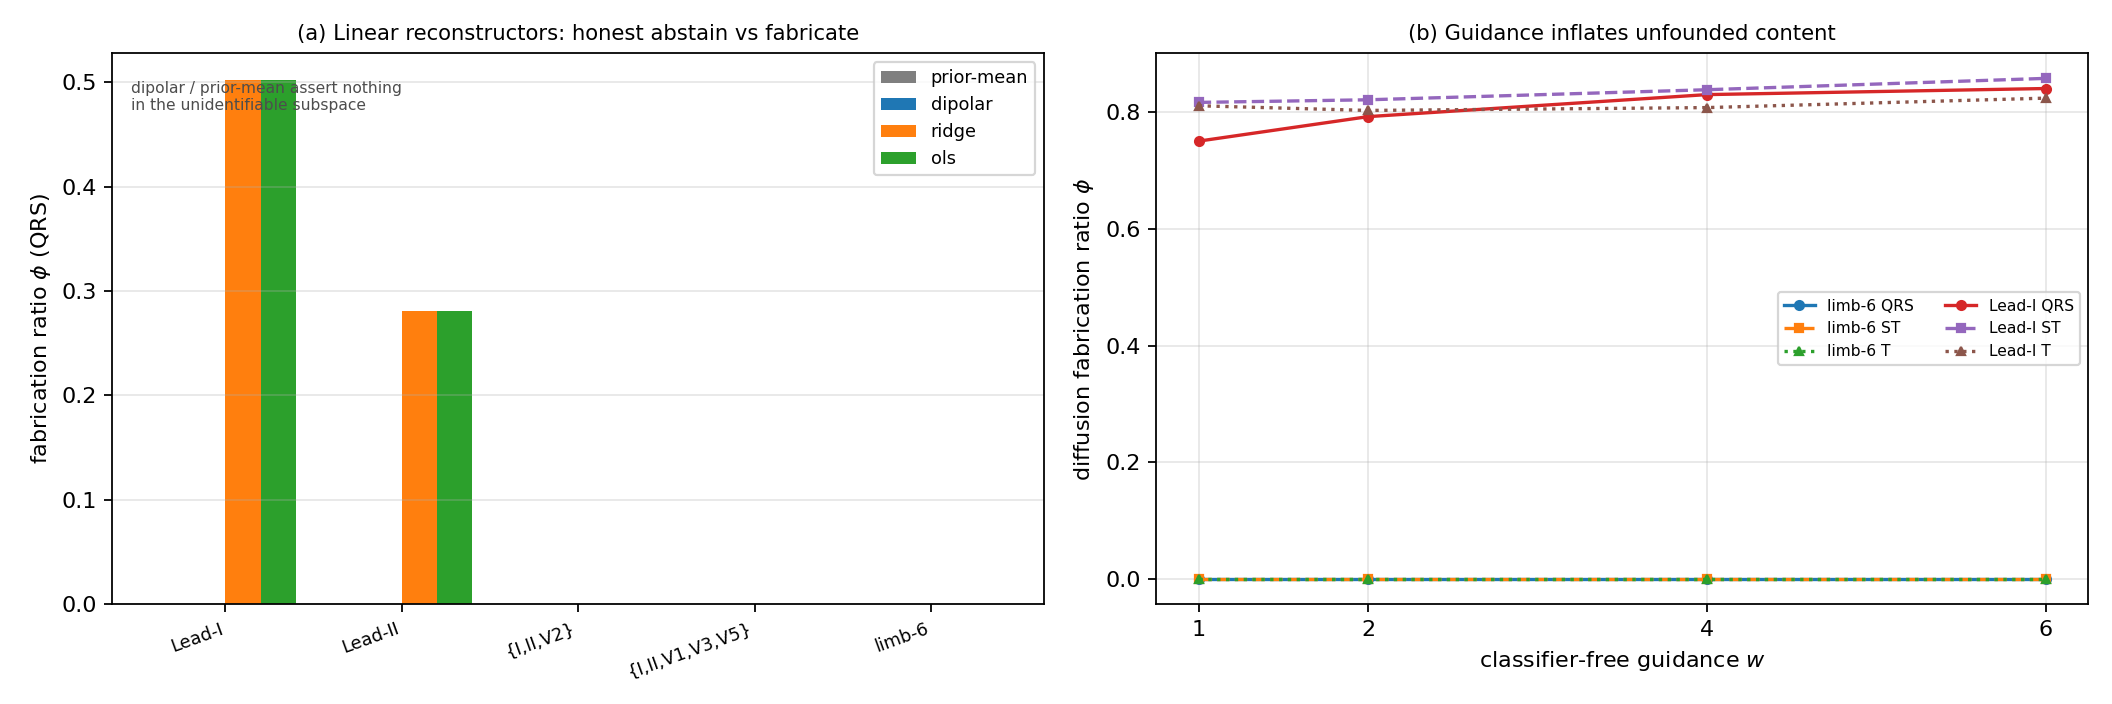
\includegraphics[width=\linewidth]{../results/fabrication_audit_figure.png}
  \caption{\textbf{Null-space dipolar fabrication audit} (ground-truth-free). $\phi$ = fraction of a
  reconstruction's dipolar energy in the certified-unrecoverable subspace $\bm Q$. (a) Linear
  reconstructors: dipolar/prior-mean abstain ($\phi{=}0$); single-lead ridge/OLS fabricate; on
  observation sets that span the dipole (incl.\ limb-6) even ridge/OLS abstain. (b) The diffusion
  model fabricates most of its dipolar content on a single lead and fabrication \emph{grows with
  classifier-free guidance} $w$, while abstaining on limb-6. Regenerated from
  \texttt{results/fabrication\_audit.json}, \texttt{fabrication\_diffusion.json}.}
  \label{fig:fab}
\end{figure}